\chapter{Teoretické východiská práce} 

\section{Úvod do fuzzy dát}
%todo pridat do zoznamu zdrojov a potom to tuto v tejto kapitole citovať
%z knihy Projektovanie systémov pre podporu rozhodovania na základe neurčitých dát, Vitaly Levasheko, Elena Zaitseva, Štefan Kovalík, Vydala Žilinská univerzita v Žiline/Edis-vydavateľstvo ŽU, 2013, ISBN 978-80-554-0680-0
%5 strana
Metódy a algoritmy využívané v súčasných systémoch pre podporu rozhodovania by mali brať do úvahy možnú nestochastickú neurčitosť vstupných dát, spôsobenú nedostatočnou presnosťou merania. Jeden z prístupov, ktorý berie do úvahy neurčitosť, je vyjadrenie vstupných hodnôt pomocou neurčitých fuzzy dát alebo pomocou viachodnotových dát. 
Matematickým aparátom spracovania neurčitých dát a viachodnotových dát je fuzzy logika a viac hodnotová logika. \cite{levashenkoProj}%, TODO PRESTYLIZOVAT
\paragraph{}
%6 strana
Neurčité dáta sa reprezentujú pomocou lingvistických premenných, ktorých hodnoty patria do konečnej množiny. 
%9 strana
Lingvistické premenné sa javia ako jeden z často používaných spôsobov vyjadrenia hodnôt, opisovaných kvantitatívnymi 
%10 strana
alebo kvalitatívnymi veličinami. Kvalitatívne veličiny sa v mnohých prípadoch javia ako výsledok formalizácie expertných odhadov. 
%10 strana = kapitola 1.1 kapitola o fuzzy dáta a expertné odhady. 
Každý objekt alebo proces sa opisuje skupinou ukazovateľov. V modeloch pre podporu rozhodovania sa využívajú ukazovatele, ktoré nadobúdajú hodnoty z množiny reálnych čísel. \cite{levashenkoProj}

Použitie reálnych čísel je zložité na presné meranie hodnôt ukazovateľa,dostupnosti nameraných dát, a relatívne vysoké náklady na meranie presných hodnôt ukazovateľov. Nie sú algoritmy a metódy výpočtu na výpočet presných hodnôt ukazovateľa. Ukazovatele reálnych hodnôt obsahujú zbytočne podrobnú informáciu, a nemôžu byť základom pre výber rozhodnutia. Aplikovaním lingvistického prístupu sa zabezpečuje spracovanie neurčitej fuzzy informácie v rozhodovacích úlohách. Lingvistický prístup umožnuje formalizovať neurčité fuzzy pojmy pomocou fuzzy množín a premenných, a spracovávať ich cez teóriu fuzzy logiky. 



% tieto pojmy asi su aj v Zadeh1965, Zadeh1996 , citujem ich doslovne z knihy = Projektovanie systemov.. 
\subsection{Definície}

Nech $ X = \left\lbrace x \right\rbrace$ je množina prvkov x. 


\paragraph*{Definícia 1.} 
  Fuzzy množina $A \subset X $ je predstavovaná množinou dvojíc $ \left\lbrace \left( x, \mu_A \left( x \right) \right) \right\rbrace  $, kde $ x \in X$ a $ \mu_A : X \longrightarrow \left\langle 0, 1\right\rangle $ je funkcia príslušnosti, ktorá predstavuje subjektívnu mieru príslušnosti elementu x k množine A. 
Veličina $\mu_A\left( x\right) $ nadobúda hodnoty od nuly, ktorá označuje absolútnu nepríslušnosť po hodnotu jedna, ktorá hovorí o absolútnej príslušnosti elementu x do fuzzy množiny A. \cite{Zadeh1965, levashenkoProj}
% toto bolo doslova asi citovane zo 
%Zadeh L., Fuzzy sets. Information and Control, vol.8, 1965, pp. 338-353. 

%12 strana knihy o projektovani systemov
Ak je fuzzy množina A definovaná na konečnej univerzálnej množine 
\\
 $X = \left\lbrace x_1, x_2, ... , x_i, ..., x_n\right\rbrace $, potom je vhodné označiť ju nasledovne
$$
A = \left\lbrace 
\left( x_1, \mu_A\left( x_1\right)  \right) , 
\left( x_2, \mu_A\left( x_2\right)  \right) , ... , 
\left( x_i, \mu_A\left( x_i\right)  \right) , ... , 
\left( x_n, \mu_A\left( x_n\right)  \right) 
 \right\rbrace , 
$$ 
kde $\left( x_i, \mu_A\left( x_i\right)  \right)$ - je dvojica tvorená elementov $x_i$ a jeho funkciou príslušnosti, nazývaná singleton. \cite{levashenkoProj}

%%tieto definicie su na strane 12, a su citovane z knihy, a aj Kaufmann1985, Klir1995, Navara2011

\paragraph*{Definícia 2. }
Fuzzy premenná je definovaná trojicou $\left( \alpha, X, A \right) $, kde 
$\alpha $ - je meno fuzzy premennej, 
 $X=\left\lbrace x \right\rbrace$ - je množina, tvoriaca definičný obor premennej x, 
 A - je fuzzy podmnožina fuzzy množiny X, pre každý prvok ktorej je definovaná funkcia $\mu_A\left( x\right)$, udávajúca stupeň príslušnosti daného elementu x do množiny A.  \cite{levashenkoProj}

\paragraph*{Definícia 3.}
Lingvistická premenná je definovaná päticou 
$
\left(
\beta, T, X, G, M
 \right) 
$, kde 
$\beta$ - je meno lingvistickej premennej; 
T - je množina jej hodnôt $\left( termov \right) $, z ktorých každá je fuzzy premennou na množine X;
G - je syntaktické pravidlo pre tvorbu nových mien hodnôt lingvistickej premennej $\beta$;
M - je sémantická procedúra, umožňujúca transformovať novú hodnotu premennej $\beta$, určenú procedúrou G, na fuzzy premennú, t.j. vytvoriť zodpovedajúcu fuzzy množinu. \cite{levashenkoProj}


\paragraph*{Definícia 4.}
Funkcia príslušnosti $\mu_A\left( x\right)$ kvantitatívne určuje príslušnosť elementov základnej množiny uvažovaného priestoru $x \in X$ k fuzzy množine A. Hodnota A tejto funkcie značí, že element nepatrí do fuzzy množiny, hodnota 1 opisuje úplne patriaci element. Hodnoty medzi 0 a 1 charakterizujú neurčito zaradené elementy. \cite{levashenkoProj, Kaufman1985, Klir1995, Navara2011}
%todo pridat to do zoznamu literatury, plus stiahnut, a pozriet ci su tam tie definicie
%Kaufman1985
%Kaufmann A., Gupta M., Induction to fuzzy arithmetic: theory and applications. New York : Van Nostrand Reinold Co., 1985, 361 p. 
%Klir1995
%Klir G., Yuan B., Fuzzy Sets and Fuzzy Logic. Theory and Applications. Prentice Hall, 1995, 591 p. 
%Navara2011
%Navara M., Computation with fuzzy quantities. Proc. of the 7th Conf. of the European Society for Fuzzy Logic and Technology (EUSFLAT), Aix-les-Bains, France, 2011, pp. 209-214.

\paragraph*{}
Lingvistická premenná sa od číselnej premennej líši tým, že jej hodnotami nie sú čísla, ale slová alebo výroky prirodzeného alebo formálneho jazyka. Je zrejmé, že takýto 
%14 strana
kvalitatívny popis s využitím slov je menej presný ako pomocou čísel. Napriek tomu použitie lingvistickej premennej umožňuje približne opísať zložité javy, ktoré nie je možné opísať pomocou obvyklých kvalitatívnych termínov. Dôležitý aspekt lingvistickej premennej spočíva v tom, že táto premenná má vyššiu úroveň ako fuzzy premenná v tom zmysle, že hodnotami lingvistickej premennej sú fuzzy premenné.  \cite{levashenkoProj}


























\pagebreak
\section{Fuzzy prístupy}
%z knihy od michal gregor - umela inteligencia
%na strane 11 a 12 cituje v clanku ref 13

%11 strana knihy o umelej inteligenciie z od gregora
%doslovné citovanie
Fuzzy prístupy možno považovať za odpoveď na požiadavku spracovania neurčitosti, resp. nepresnosti. Táto požiadavka je veľmi rozšírená - v určitej forme sa vyskytuje prakticky v každom reálnom systéme aplikujúcom metódy umelej inteligencie - predovšetkým sa však objavuje tam, kde systémy nejakým spôsobom interagujú s človekom alebo využívajú ľudské znalosti. 
V súvislosti s neurčitosťou sa rozlišujú tri základné pojmy: \cite{gregorRef13, gregorUI}  %tuto cituje [13] (Niklesa) 
%todo prestylizovat toto!!!
\begin{itemize}
	\item \textbf{Neurčitosť} - vyplýva z nedostatočnej znalosti faktorov alebo udalosti. O neurčitosti hovoríme, že je aleatórna, ak pramení z vnútorných vlastností nejakého náhodného javu - t.j. ju principiálne nemožno odstrániť. Ak neurčitosť vyplýva z neznalosti, tak je epistemická. 
	\item \textbf{Nepresnosť} - O nepresnosti hovoríme, ak je znalosť faktov a udalosti taká kompletná ako len môže byť, ale spôsob ich vyjadrenia nie je presný alebo jednoznačný. 
	\item \textbf{Nekonzistentnosť} - O nekonzistentnosti hovoríme, ak si znalosti, resp. známe fakty navzájom odporujú. 
\end{itemize}

%12 strana knihy umela inteligencia
Ľudské znalosti vo väčšine prípadov zahŕňajú neurčitosti, nepresnosť, niekedy môžu byť aj nekonzistentné. 
Fuzzy prístupy umožňujú určitým spôsobom formalizovať a ďalej spracúvať vágne poznatky. Vágnosť možno považovať za typ nepresnosti. 
%tuto on cituje 13
 Takýto typ znalostí je ťažké a často aj nemožné vhodne formalizovať konvenčnými metódami. Fuzzy prístupy predstavujú jednu z možných ciest ako k nim pristupovať, a použiť na formalizáciu neurčitosti. \cite{gregorUI, gregorRef13}  

Teória fuzzy množín je zovšeobecnením klasickej teórie množín - fuzzy množiny sú vágne v tom či prvok patrí alebo nepatrí do množiny. 
Na fuzzy množinách možno vykonávať určité operácie čiastočne analogické s tými, ktoré sú v klasickej teórie množín. 
Fuzzy logika predstavuje prístup, ktorý zovšeobecňuje konvenčnú logiku a produkčné pravidlá zavedením tzv. lingvistických premenných a lingvistických pravidiel. 
Fuzzy logika umožňuje formulovať vágne pravidlá. 
Fuzzy aritmetika rozširuje princípy klasickej aritmetiky na vágne - fuzzy - čísla. \cite{gregorUI} 

\subsection{Teória fuzzy množín}

V klasickej teórii množín prvok môže do množiny buď patriť alebo nepatriť. Pre klasické množiny možno definovať tzv. charakteristickú funkciu. 

Charakteristická funkcia klasickej množiny S je priradenie typu \cite{gregorUI} 

\begin{equation}\label{charfunkcia}
\mu_S : U \longrightarrow \{0, 1\}
\end{equation}

Priradenie hodnoty 0 - nepatrí, alebo hodnoty 1 - patrí - ku každému prvku x $\in$ U, pričom definičný obor charakteristickej funkcie U sa nazýva univerzum. Univerzum je množina všetkých hodnôt, o ktorých rozhodujeme či do danej množiny patria, alebo nepatria. Platí $S \subseteq U$. \cite{gregorUI} 

Charakteristickú funkciu klasickej množiny možno definovať nasledovne \cite{gregorUI, gregorRef14} 
%pozri a najdi tento zdroj - Ross, T.J. Fuzzy Logic with Engineering Applications. .. alebo pozri zdroje v knihe 14

\begin{equation}\label{charfunkciafuzzy}
\mu_S (X) = 
\begin{cases}
1 &  x \in S, \\
0 &  x \notin S.
\end{cases}
\end{equation}

V teórii fuzzy množín sa zavádza rozšírenie tohto konceptu - prvok môže do množiny patriť aj čiastočne: viac alebo menej. Vágnosť je teda v otázke príslušnosti prvku ku množine. \cite{gregorUI} 

%strana 13 knihy inteligencii
\subsubsection{Stupeň príslušnosti a funkcia príslušnosti}
Mieru do akej prvok patri do fuzzy množiny sa vyjadruje stupňom príslušnosti. Nech A je fuzzy množina. Stupeň príslušnosti prvku x ku množine A označujeme $\mu_A\left( x\right) $. 
Hovoríme tiež, že $\mu_A\left( x\right) $ je funkcia príslušnosti fuzzy množiny A. \cite{gregorUI, gregorRef14} 
%toto bolo citované od neho = a on tam ma tento zdroj
%ross , T.J. Fuzzy Logic with Engineering Applications. John Wiley & Sons, 2004, secound edition ed. ISBN 0-470-86075-8. 
Funkcia príslušnosti je priradenie
\begin{equation}\label{funPrislus}
\mu_A : U \longrightarrow \left\langle 0, 1 \right\rangle 
\end{equation}
Obor hodnôt je teda v tomto prípade 
\begin{equation}\label{funPrislus}
\mu_A (X) : U \in \left\langle 0, 1 \right\rangle 
\end{equation}

Pritom rozlišujeme nasledujúce prípady: 
\begin{itemize}
	\item ak $\mu_A (x) = 0$, hovoríme, že prvok do množiny A nepatrí, 
	\item ak $\mu_A (x) = 1$, hovoríme, že prvok do množiny A patrí, 
	\item ak $\mu_A (x) \in (0, 1)$, hovoríme, že prvok patrí do množiny A čiastočne, so stupňom príslušnosti ak $\mu_A(x)$. 
\end{itemize}

Aj v tomto prípade sa dá použiť značenie $A\subseteq U$, čím sa rozumie, že množina A je definovaná na univerze U.  \cite{gregorUI} 

%strana 14 knihy umela inteligencia
\subsubsection{Spojité a diskrétne fuzzy množiny}
Fuzzy množiny možno rozdeliť podľa spojitosti na spojité a diskrétne. V prípade spojitých fuzzy množín je univerzum spojité. T.j. aj funkcia príslušnosti je spojitá. Naopak v prípade diskrétnych fuzzy množín sú univerzum aj funkcia príslušnosti diskrétne. Obor funkcie príslušnosti je spojitý v oboch prípadoch.  \cite{gregorUI} 


\subsubsection{Spôsoby zápisu fuzzy množín}
Fuzzy množiny možno zapísať buď diskrétne alebo spojito.

%v knihe o umelej inteligencii je to vedene ako 1 ref. 
%SPALEK.J - JANOTA. A - BLAŽOVIČOVÁ, M. - PŘIBYL, P. Rozhodovanie a riadenie s podporou umelej inteligencie. Žilinská univerzita v Žiline/EDIS, 2005. ISBN 80-8070-354-X. 
V prípade, že ide o diskrétnu fuzzy množinu, možno použiť nasledujúci zápis \cite{gregorref1, gregorUI}

\begin{equation}\label{disk0}
A = \{\mu_A(x_1)/x_1, \mu_A(x_2)/x_2, ... , \mu_A(x_n)/x_n\}, 
\end{equation}
kde n je počet prvkov, $x_i in U : \forall_i = 1, 2, ..., n$ sú prvky univerza a $\mu_A(x_i)$sú ich stupne príslušnosti.

%14,15 strana
Ďalšia konvencia zápisu diskrétnych fuzzy množín je  \cite{gregorUI} 

\begin{equation}\label{disk1}
A = \{\mu_A(x_1)/x_1 + \mu_A(x_2)/x_2, ...  + \mu_A(x_n)/x_n\}, 
\end{equation}

\begin{equation}\label{disk2}
A = \left\lbrace 
\left( x_1; \mu_A\left( x_1\right)  \right) , 
\left( x_2; \mu_A\left( x_2\right)  \right) , ... , 
\left( x_n; \mu_A\left( x_n\right)  \right) 
\right\rbrace , 
\end{equation}

\begin{equation}\label{disk3}
A = 
\sum\limits_{i=1} \mu_A(x_i)/x_i . 
\end{equation}

Spojité fuzzy množiny možno reprezentovať výrazom v tvare \cite{gregorref1}
\begin{equation}\label{disk4}
A = \int_{U}^{}  \mu_A(x)/xdx . 
\end{equation}
%16 strana
\subsubsection{Singleton}
Špeciálnym typom fuzzy množiny je tzv. singleton. Ide o taký typ fuzzy množiny, pre ktorý iba jeden bod univerza má stupeň príslušnosti väčší ako 0. 
Nech teda A je fuzzy množina definovaná na univerze U. Potom fuzzy množinu A považujeme za singleton, ak existuje bod $x_0 \in U$ taký, že platí \cite{gregorUI} 
\begin{equation}\label{singleton0}
\mu_S (X) = 
\begin{cases}
b &  x = x_0 \\
0 &  inak
\end{cases}
\end{equation}
 $$ b \in \left(  0, 1 \right\rangle $$
Singleton možno zapísať obdobným spôsobom ako diskrétnu fuzzy množinu a to je \cite{gregorUI} 
\begin{equation}\label{singleton1}
A = \left\lbrace b/x_0 \right\rbrace , 
\end{equation}
\begin{equation}\label{singleton2}
A = \left\lbrace \left( x_0 ; b \right) \right\rbrace 
\end{equation}

%26 strana knihy o umelej inteligencii 
\subsection{Fuzzy logika}
\subsubsection{Lingvistická premenná}
Lingvistická, resp. jazyková premenná je zvláštnym typom premennej, ktorá sa od numerických premenných odlišuje tým, že jej hodnoty - tzv. lingvistické hodnoty - nie sú čísla, ale slovné výrazy. Pritom každej lingvistickej hodnote je priradený význam, t. j. určitá fuzzy množina definovaná na spoločnom univerze. \cite{gregorUI}

\subsubsection{Fuzzy inferenčný systém}
Lingvistické premenné možno využiť na odvodzovanie a získať z nich výstupné ostré hodnoty (t.j. presné číselné hodnoty). 
Inferenčný systém je štruktúra umožňujúca odvodzovať na základe vopred daných pravidiel a známych faktov nové fakty. V prípade fuzzy inferenčného systému (FIS) možno pri formulácii pravidiel navyše využiť lingvistické premenné a hodnoty. Medzi najznámejšie metódy fuzzy inferencie patrí Mandaniho inferencia. \cite{gregorUI}
V prípade, že sa má fuzzy inferenčný systém použiť ako jadro regulátora, je potrebné, aby jeho vstupmi a výstupmi boli ostré hodnoty. FIS umožňujú aj prevod z ostrých (presne číselných) vstupov na lingvistické hodnoty a naopak. \cite{gregorUI}
Bloková schéma na Obr. \ref{fig:fis} zobrazuje hlavné komponenty fuzzy inferenčného systému: F - fuzzifikácia, inferencia, báza pravidiel, D - defuzzifikácia. 
%strana 28
\begin{figure}[h]
	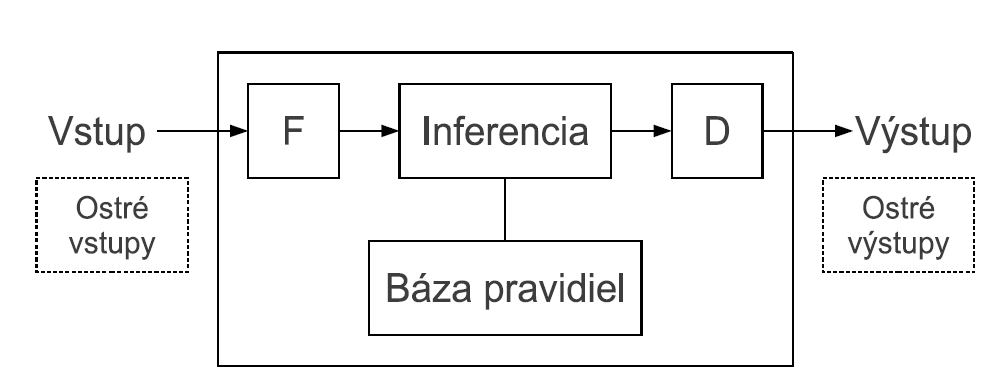
\includegraphics[width=0.75\textwidth]{obrazky/obrazok1}
	\centering
	\caption{Fuzzy inferenčný systém - bloková schéma.\cite{gregorUI}}
	\label{fig:fis}
\end{figure}

\subsubsection{Báza pravidiel}
Fuzzy inferenčný systém pri odvodzovaní nových faktorov vychádza z určitých vopred daných pravidiel. Tie sú združené v báze pravidiel. Pravidlá majú vo všeobecnosti nasledujúci tvar \cite{gregorUI, gregorRef19, gregorref1}
%tuto cituje 19 zdroj
\begin{quote}\centering
         \textbf{AK} (predpoklad)   \textbf{POTOM} (dôsledok), resp. \\
         \textbf{IF} (antecedent)  \textbf{THEN} (consequent).
\end{quote}
Predpoklad sa pritom skladá z termov nasledujúceho tvaru \cite{gregorUI}
\begin{equation}\label{baza1}
X \hspace{0.2cm} is \hspace{0.2cm}  A_i , 
\end{equation}
kde X je lingvistická premenná a $A_i$ je i-tá lingvistická hodnota tejto premennej. 

% 28-29 strana
\subsubsection{Fuzzifikácia}
Z blokovej schémy na Obr. \ref{fig:fis} je zrejmé, že do fuzzy inferenčného systému môžu vstupovať ostré hodnoty. Aby bolo možné vykonať porovnanie podľa (\ref{baza1}), ostrú vstupnú hodnotu je potrebné previesť na fuzzy množinu. Tento proces sa nazýva fuzzifikácia. Fuzzifikácia je prevod ostrej hodnoty x na fuzzy množinu $L_x$, pričom výstupom je často singleton \cite{gregorUI}
\begin{equation}\label{fuzzysingle1}
L_x = \left\lbrace1/x\right\rbrace .  
\end{equation}
Majme term v tvare podľa (\ref{baza1}). Ak ostrá hodnota premennej je x a jej fuzzifikovaná hodnota  $L_x$, potom takýto term možno vyhodnotiť jednoducho pomocou zvolenej T-normy (analógia prieniku). Ako T-norma sa v tomto prípade spravidla používa operátor minima  $T_m(a, b)=min(a, b)$. Ak sa aplikuje na dané operandy vznikne \cite{gregorUI}
\begin{equation}\label{fuzzimin}
\alpha_x = min(L_x, A^{i}) \forall x \in U, 
\end{equation}
kde $\alpha_x$ možno považovať za mieru platnosti tvrdenia (\ref{baza1}). 
Vzhľadom na vlastnosti singletonov možno tento postup zjednodušiť na 
\begin{equation}\label{fuzziminsingle}
\alpha_x = \left\lbrace \mu_{A^i}(x)/x\right\rbrace , 
\end{equation}
Keďže $\alpha_x$ je tiež singleton, tak stačí, ak sa vyjadrí iba ako $\mu_{A^i}(x)$, čo je ostré číslo. 
Fuzzifikácia v praxi je vyhodnotenie miery platnosti predpokladu X is A (\ref{baza1}) na základe znalosti ostrej hodnoty x premennej X. Miera platnosti takého predpokladu je pritom ekvivalentná stupňu príslušnosti ostrej hodnoty x ku fuzzy množine A, čiže  $\mu_{A}(x)$. \cite{gregorUI}  

%treba definovať T=normu?????? 
\pagebreak








\pagebreak
\section{Transformácia číselných hodnôt na lingvistické premenné}
%todo uplne prestylizovať do ľudskej reči
Transformácia číselných premenných na lingvistické predpokladá vzťah medzi kombináciou ich hodnôt a stupnicou s konečným počtom m intervalov sa nazýva diskretizáciou. 
%tuto cituju Catlett1991, Ching1995, Kotsiantis2006 
%todo zdroje
Pritom sa každý interval asociuje s hodnotou lingvistickej premennej (termom). Proces diskretizácie predpokladá transformáciu kvantitatívnych dát na kvalitatívne. \cite{levashenkoProj, Catlett1991}


Vo všeobecnom prípade diskretizácia zmenšuje objem dát a nevedie k zníženiu klasifikačnej presnosti a spoľahlivosti hodnôt  využívaných v systémoch pre podporu rozhodovania. Naopak, takéto diskrténe hodnoty adekvátne ohodnocujú ukazovatele a sú stabilnejšie vzhľadom na zmeny a metodiky merania. 
%tuto cituju Lui2002
%todo zdroje
\cite{levashenkoProj, Lui2002}

Úloha diskretizácie sa formuluje nasledovne. 
%tuto cituju Garcia2013
%todo zdroje
\subsection{Definícia úlohy diskretizácie}
Majme množinu pozostávajúcu z N príkladov. Každý príklad obsahuje množinu vstupných číselných premenných. Nech niektorá vstupná číselná premenná X v týchto príkladoch nadobúda hodnoty v rozsahu od $x_min$ po $x_max$. Potom diskretizáciou tejto spojitej premennej sa nazýva proces rozkladu jej hodnôt na m diskrétnych intervalov
\begin{equation}\label{dkiskr}
D =\left\lbrace
\left\langle d_0, d_1 \right) , 
\left\langle d_1, d_2 \right) , ... , 
\left\langle d_{m-1}, d_m \right\rangle 
 \right\rbrace, 
\end{equation} 
kde $d_0$ je minimálna hodnota $x_min$ tejto premennej, $d_m$ je maximálna hodnota $x_max$ premennej a platí $d_i < d_{i+1}$, pre i = 0, 1, ... m-1. 
Pritom, $P = \left\lbrace d_1, d_2, ..., d_{m-1} \right\rbrace$ je množina bodov rezu premennej X.    \cite{levashenkoProj, Garcia2013}

%todo pridaj Chelbus1998 do zdrojov

\subsection{Metódy diskretizácie}
Získanie optimálnej diskretizácie prestavuje NP-zložitú úlohu. \cite{levashenkoProj, Chelbus1998} Existencia obrovského množstva metód diskretizácie je vysvetliteľná rozmanitou povahovou vstupných dát a požiadaviek na ich spracovanie. Výber použitej metódy diskretizácie určuje úspešnosť ich budúceho spracovania. Na výber metódy má vplyv množstvo parametrov.  \cite{levashenkoProj}
\begin{enumerate}
	\item \textbf{Počet intervalov rozkladu.}  Príliš malý počet intervalov spôsobuje nepresnosti a chyby vo vstupných dátach a vedie k hrubému vyjadreniu výsledku. Na druhej strane rozklad vstupných dát na príliš veľký počet intervalov spôsobuje prílišnú detailizáciu a následne vedie k tomu, že spracovanie takýchto dát je pomalé a neefektívne  \cite{levashenkoProj, Catlett1991}%tuto cituju Catlett1991
	\item \textbf{Nesúlad s výsledkom. }  Nesúlad s výsledkom sa objasňuje vznikom neočakávaných chýb v procese diskretizácie. Tieto chyby súvisia s nepresnosťami diskretizácie vstupných dát a vo vzťahu medzi týmito diskretizovanými hodnotami a hodnotami výstupného atribútu.  \cite{levashenkoProj}
	\item \textbf{Presnosť rozkladu.}  Predpokladá, že úspešný algoritmus diskretizácie, skonštruovaný na základe výberu tréningových dát, pracuje bez podstatného zníženia kvality aj na všetkých nasledujúcich dátach.  \cite{levashenkoProj}
	\item \textbf{Časové ohraničenia.}  V prípade statických procesov, kedy požiadavka diskretizácie výučbovej množiny vzniká iba raz, nie je čas výpočtu dôležitým parametrom. Avšak pri dynamických procesoch, keď sa etapa diskretizácie výučbovej množiny opakuje mnohokrát, je čas spracovania kritickým parametrom.  \cite{levashenkoProj}
\end{enumerate}

Proces transformácie reálnych hodnôt na konečný počet intervalov a reprezentovanie každého intervalu s diskrétnou hodnotou predstavuje proces, ktorý je už dosť dobre preskúmaný. Vykonaná analýza odhalila rad základných kritérií klasifikácie existujúcich metód diskretizácie. Podrobnejšie je prehľad a analýza existujúcich metód diskretizácie uvedená v prácach \cite{Lui2002, Liu2004, Singh2007, Bakar2009, Yang2010, Garcia2010, Garcia2013} . 

%20-24 strana
\subsubsection{Statické a dynamické metódy diskretizácie}
Kritérium uvažuje klasifikáciu metód na základe opakovateľnosti procesu diskretizácie. 

Statické metódy sa realizujú v tvare predbežnej samostatnej etapy spracovania vstupných dát a nezávisia od spôsobu následného využitia diskretizovaných hodnôt. 

Dynamická diskretizácia je obvykle zabudovaná do mechanizmu inteligentného spracovania dát a využíva sa napríklad pri konštrukcii rôznych klasifikátorov. \cite{levashenkoProj}
%todo odpisat tie priklady algoritmov... 

\subsubsection{Globálne a lokálne metódy diskretizácie}
Kritérium berie do úvahy úplnosť množiny a dostupnosť vstupných hodnôt, použitých v procese diskretizácie. 

Globálne metódy diskretizácie spracovávajú vstupnú množinu hodnôt číselného atribútu počas etapy predbežného spracovania. 

Lokálne metódy predpokladajú diskretizáciu dát súčasne s inými metódami ich spracovania. K tomuto typu patria dynamické metódy diskretizácie, ktoré zisťujú body rezu v rámci vnútorných operácií algoritmov spracovania dát a nemajú prístup k úplnej množine vstupných dát. \cite{levashenkoProj}

\subsubsection{Metódy jednorozmernej, mnohorozmernej diskretizácie}
Kritérium slúži na klasifikáciu metód diskretizácie na základe počtu súčasne spracovaných atribútov. 

V jednorozmernej diskretizácii sa každý číselný atribút transformuje na lingvisticky nezávisle od hodnôt iných atribútov. 

Metódy mnohorozmernej diskretizácie predpokladajú súčasné spracovanie všetkých číselných atribútov. 
Vo výsledku rozklad hodnôt číselných atribútov na intervaly vykonáva s prihliadnutím na množný vzájomný vplyv vstupných atribútov jedného na druhý. \cite{levashenkoProj}

\subsubsection{Diskretizácia bez učitela, s učiteľom}
Kritériium rozlišuje neriadenú diskretizáciu bez učiteľa alebo riadenú diskretizáciu s učiteľom. 

Diskretizácia bez učiteľa určuje body rezu iba na základe analýzy vstupných atribútov. Hodnoty výstupného atribútu sa pritom neberú do úvahy. 

Diskretizácia s učiteľom pri rozklade vstupného atribútu na niekoľko intervalov navyše zisťuje vzťah medzi hodnotami vstupných atribútov a im zodpovedajúcimi hodnotami výstupných atribútov. Výsledkom použitia diskretizácie s učiteľom ej možnosť takého rozdelenia vstupného atribútu, kedy rôznym intervalom zodpovedajú rôzne hodnoty výstupného atribútu. Využitie diskretizácie s učiteľom umožňuje automaticky určovať najlepší počet intervalov a body rozdelenia pre každý atribút s perspektívou realizácie budúcej klasifikácie alebo klusterizácie výstupného atribútu. %Dougherty1995
\cite{levashenkoProj}

\subsubsection{Priame a inkrementálne metódy diskretizácie}
Kritérium predpokladá klasifikáciu podľa spôsobu získania intervalov. 

Metódy priamej diskretizácie naraz rozdelia vstupnú množinu na m intervalov. Využitie týchto metód na začiatku vyžaduje určenie veličiny m. V každom kroku spracovania vyberajú tieto metódy niekoľko bodov rezu. 

Na druhej strane metódy postupnej diskretizácie predpokladajú hľadanie najlepšieho kandidáta na bodu rezu. 
\cite{levashenkoProj}
\subsubsection{Neparametrické a parametrické metódy diskretizácie }
Kritérium predstavuje variant predchádzajúceho kritéria a určuje spôsob získania počtu intervalov pre každý atribút. 

Neparametrické metódy určujú najlepší počet intervalov pre každý atribút. 

Parametrické metódy predpokladajú, že počet intervalov je už apriórne zadaný. 
\cite{levashenkoProj}

\subsubsection{Metódy zlučovacej a rozdeľovacej diskretizácie}
Kritérium klasifikuje metódy diskretizácie v závislosti od spôsobu spracovania vstupných hodnôt - zlučovanie alebo rozdeľovanie. 

Zlučovacia (merging) diskretizácia predpokladá postupné pridávanie bodov rezu a jeho výsledkom je rozklad na menšie intervaly. 

Rozdeľovacia (splitting) diskretizácia spočíva v odstraňovaní bodov rezu, čo vedie k postupnému zlučovaniu skupiny susedných intervalov do väčšieho intervalu. 

Opakovanie procesov rozdeľovania alebo zlučovania sa riadi ukončovacím kritériom. 

Ako primitívne kritérium ukončenia vystupuje napríklad apriórne zadaný počet intervalov. 

Ako zložité kritérium sa používa napríklad minimálna chyba klasifikácie. Toto kritérium je prípustné iba pre metódy inkrementálnej diskretizácie. 

Sú známe aj metódy diskretizácie, ktorých činnosť je založená na zlučovaní alebo rozdeľovaní niekoľkých intervalov. 
Hybridné metódy počas činnosti striedajú spájanie a rozdeľovanie. \cite{levashenkoProj}

\subsubsection{Metódy diskretizácie podľa použitého parametra}
Kritérium klasifikuje metódy diskretizácie podľa použitého parametra porovnania rozličných variantov rozdelenia. 

Metóda založená na informačných ukazovateľoch často využíva pojem entropie a iné ukazovatele, založené na pojmoch teórie informácie. 

Štatistické metódy berú do úvahy mieru závislosti (korelácie) medzi atribútmi. 

Metódy, berúce do úvahy frekvenčné charakteristiky, patria k najjednoduchším metódam diskretizácie. V týchto metódach a každý interval určuje vopred, určením apriórne zadaného počtu hodnôt. 

Kolekcia metód využívajúcich chybu klasifikácie, presnosti klasifikácie. \cite{levashenkoProj}

\subsubsection{Metódy diskretizácie vytvárajúce nepretínajúce a pretínajúce sa intervaly}
Klasifikácia na základe vlastností získaných intervaloch. 

K metódam diskretizácie vytvárajúce nepretínajúce sa intervaly patria doteraz všetky vymenované metódy diskretizácie. Tieto metódy vytvárajú v procese diskretizácie m diskrétnych intervalov
$
\left\langle d_0, d_1 \right) , 
\left\langle d_1, d_2 \right) , ... , 
\left\langle d_{m-1}, d_m \right\rangle 
$
pre ktoré platia nerovnosti $d_i < d_{i+1}$, pre i = 0, 1, ... m-1. 

Pre metódy diskretizácie, ktoré pretínajú intervaly nemusí platiť nerovnosť. K takýmto metódam patrí fuzzy diskretizácia. \cite{levashenkoProj}

\subsection{Príklady algoritmov metód diskretizácie}


% Fig. 1 illustrates a comparison network where each node corresponds to a discretization algorithm and a directed vertex between two nodes indicates that the algorithm of the start node has been compared with the algorithm of the end node. The direction of the arrows is always from the newest method to the oldest, but it does not influence the results. The size of the node is correlated with the number of input and output vertices. We can see that most of the discretizers are represented by small nodes and that the graph is far from being complete, which has prompted the present paper.
Obrázok  \ref{fig:obrazok2} ilustruje porovnávaciu sieť, v ktorej každý uzol zodpovedá algoritmu diskretizácie a smeruje na vrchol medzi dvoma uzlami. Označuje, že algoritmus počiatočného uzlu bol porovnávaný s algoritmom koncového uzla. Smer šípok je vždy od najnovšieho spôsobu až po najstaršie. Veľkosť uzla je v korelácii s počtom vstupných a výstupných vrcholov. \cite{Garcia2013} Obrázok \ref{fig:obrazok3} zobrazuje kategorizáciu hierarchie metód diskretizácie. 

\begin{figure}
	\centering
	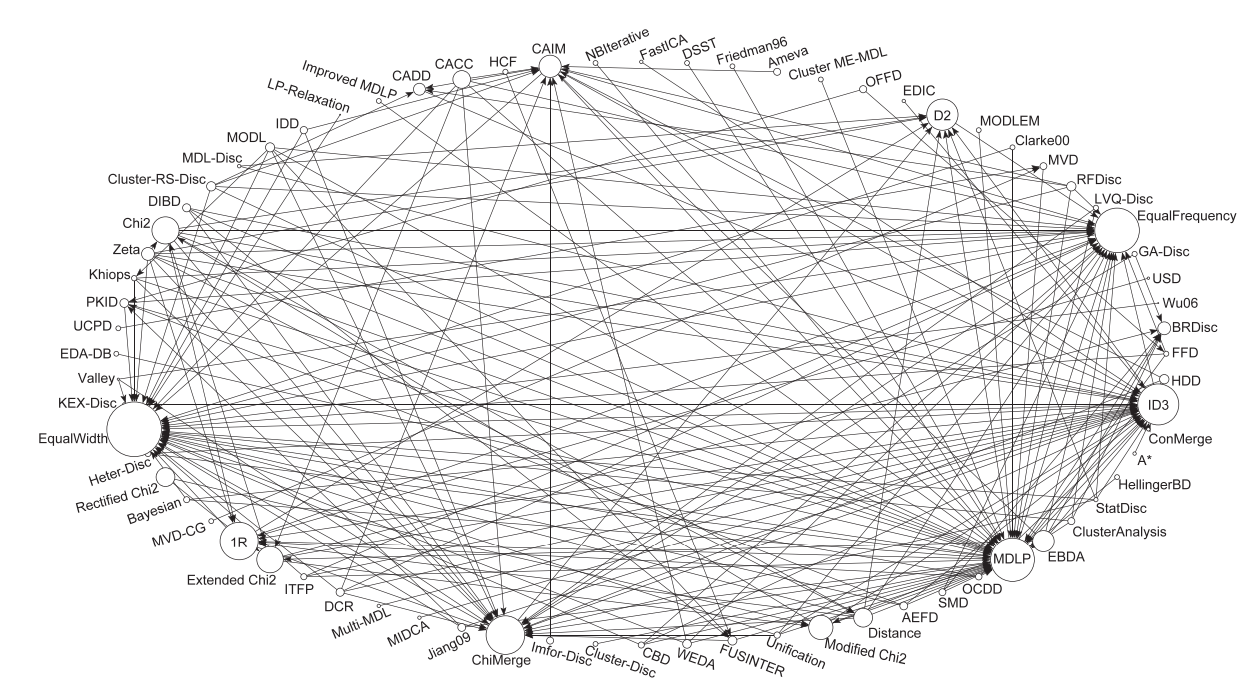
\includegraphics[width=1\linewidth]{obrazky/obrazok2}
	\caption{Porovnávacia sieť metód diskretizácie}
	\label{fig:obrazok2}
\end{figure}

\begin{figure}
	\centering
	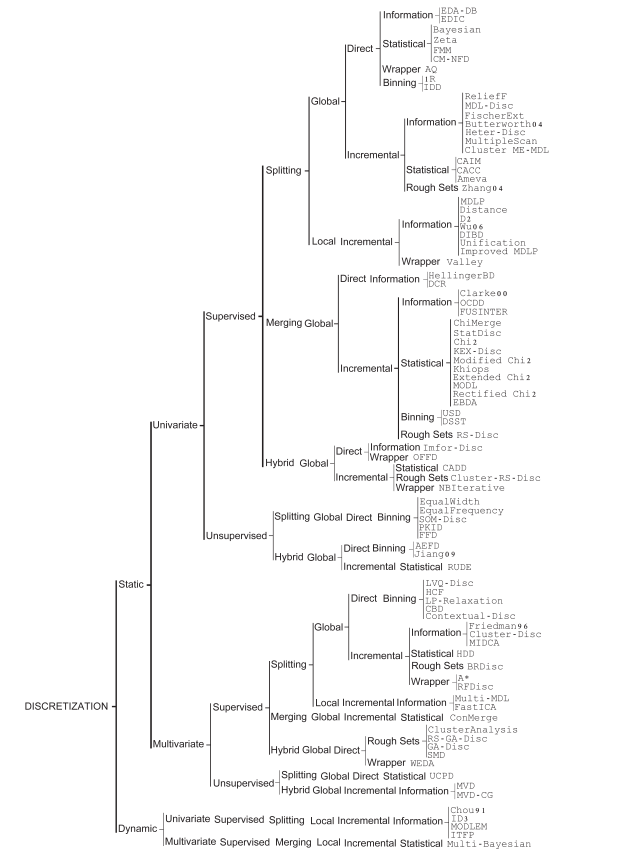
\includegraphics[height=1.36\linewidth]{obrazky/obrazok3}
	\caption{Taxonómia metód diskretizácie}
	\label{fig:obrazok3}
\end{figure}


\begin{table}[h!]
	\centering
	\begin{tabular} { |p{5cm}|p{10cm}| }
		\hline 
		\textbf{Metóda diskretizácie} & \textbf{Príklady algoritmov} \\ 
		\hline 
		Statická & ChiMerge, MDLP, Chi2, RFDisc, UnDisc, CDisc, ME-MDL, ImformDisc, ImpMDLP \\ 
		\hline 
		Dynamická & ID3 a C45, MultiBayesian, MODLEM, ITFP \\ 
		\hline 
		Globálna  & EqualWidth a EqualFrequency, ChiMerge, Chi2, CAIM, RFDisc, UnDisc, ME-MDL, EBDA, ImforDisc \\ 
		\hline 
		Lokálna & MDLP, ID3 a C45, ImpMDLP \\ 
		\hline 
		Jednorozmerná & EqualWidth a EqualFrequency, MDLP, UnDisc, EBDA, ME-MDL, ImformDisc \\ 
		\hline 
		Mnohorozmerná & MVD, Multi-MDL, UCPD, MIDCA, WEDA, RFDisc, SMD, CBD \\ 
		\hline 
		Neriadená (bez učiteľa)  & EqualWidth a EqualFrequency, MVD, UnDisc, FFD \\ 
		\hline 
		Riadená (s učiteľom) & ChiMerge, MDLP, ID3 a C45, Chi2, WEDA, RFDisc, CDisc, EBDA, ME-MDL, ImforDisc, ImpMDLP \\ 
		\hline 
		Priama & UCPD, WEDA \\ 
		\hline 
		Inkremetálna (postupná) & ChiMerge, ID3 a CD45, Chi2, MVD, RFDisc, EBDA, ImpMDLP \\ 
		\hline 
		Neparametrická & MDLP, USD, CAIM \\ 
		\hline 
		Parametrická & ChiMerge, CADD \\ 
		\hline 
		Zlučovacia & ChiMerge, EBDA \\ 
		\hline 
		Rozdeľovacia & MDLP, RFDisc, CDisc, ME-MDL, ImpMDLP \\ 
		\hline 	Súčasná & HBD, IDD \\ 
		\hline 
		Hybridná  & CADD, WEDA, ImforDisc \\ 
		\hline 
		Informačných ukazovateľov & ID3 a C45, MDLP, DbEr, ME-MDL, ImforDisc, ImpMDLP, GINI \\ 
		\hline 
		Štatistických ukazovateľov & ChiMerge, Zeta, Chi2, EBDA, MODL \\ 
		\hline 
		Frekvenčných charakteristík & EqualWidth a EqualFrequency, UnDisc \\ 
		\hline 
		Presnosti klasifikácie & Valley, NBIterative, RFDisc \\ 
		\hline 
	\end{tabular} 
	\caption{Tabuľka príkladov algoritmov jednotlivých metód diskretizácie.}
	\label{table:1}
\end{table}
 
V tabuľke \ref{table:1} sú vypísané príklady algoritmov jednotlivých metód diskretizácie. 
Vlastnosti niektorých známych algoritmov metódy diskretizácie. 
\begin{itemize}
	\item EqualWidth a EqualFrequency - globálny, jednorozmerný, založený na frekvenčných charakteristikách.\cite{Wong1987} 

\item
ChiMerge - statický, globálny, riadený, inkrementálny, parametrický, zlučovací, založený na štatistických ukazovateľov.
\cite{Keber1992} 
\item
ID3 a C45 - dynamický, lokálny, riadený, inkrementálny, založený na informačných ukazovateľov. 
\cite{Quinlan1993} 

\item
MDLP - statický, jednorozmerný, riadený, neparametrický, rozdeľovací, založený na informačných ukazovateľov.
\cite{Fayyad1993} 
\item
Valley - založený na presnosti klasifikácie. 
\cite{Ventura1994} 
\item
NBIterative - založený na presnosti klasifikácie. 
\cite{Pazzani1995} 

\item
CADD - parametrický, hybridný. 
\cite{Ching1995} 
\item
Chi2 - statický, globálny, riadený, inkrementálny, založený na štatistických ukazovateľov.
\cite{Liu1997} 
\item

Zeta - založený na štatistických ukazovateľov. 
%Ho1997
\cite{Ho1997} 
\item
MultiBayesian - dynamický 
%Monti1998
\cite{Monti1998} 
\item
MODLEM - dynamický
%Grzymala2001
\cite{Grzymala2001} 
\item
MVD - mnohorozmerný, neriadný, inkrementálny. 
%Bay2001
\cite{Bay2001} 
\item
USD - neparametrický. 
%Giraldez2002
\cite{Giraldez2002} 
\item
CAIM - globálny, neparametrický. 
%Kurgan2004
\cite{Kurgan2004} 
\item
MIDCA - mnohorozmerný. 
%Chao2005
\cite{Chao2005} 
\item
UCPD - mnohorozmerný, priamy. 
%Mehta2005
\cite{Mehta2005} 
\item
Multi-MDLP - mnohorozmerný.
%Ferrandiz2005
\cite{Ferrandiz2005} 
\item
MODL - založený na štatistických ukazovateľov. 
%Boulle2006
\cite{Boulle2006} 
\item
ITFP - dynamický
%Au2006
\cite{Au2006} 
\item
HBD - súčasné zlučovanie/rozdeľovanie niektoľkých intervalov. 
%Lee2007
\cite{Lee2007} 
\item
WEDA - mnohorozmerný, riadený, priamy, hybridný. 
%Flores2007
\cite{Flores2007} 
\item
IDD - súčasné zlučovanie/rozdeľovanie niektoľkých intervalov. 
%Ruiz2008
\cite{Ruiz2008} 
\item
DbEr - založený na informačných ukazovateľov. 
%Hu2008
\cite{Hu2008} 
\item
RFDisc - statický, globálny, mnohorozmerný, riadený, inkrementálny, rozdeľovací, založený na presnosti klasifikácie.
%Berrado2009
\cite{Berrado2009} 
\item
UnDisc - statický, globálny, jednorozmerný, neriadný, založený na frekvenčných charakteristikách.
%Jiang2009
\cite{Jiang2009} 
\item
GINI 
%Jin2009 - založený na pojmoch teórie informácie. 
\cite{Jin2009} 
\item
FFD - neriadný. 
%Yang2009a
\cite{Yang2009a} 
\item
SMD - mnohorozmerný. 
%Jiang2009
\cite{Jiang2009} 
\item
CDisc - statický, riadený, rozdeľovací, 
%Nemmiche2010
\cite{Nemmiche2010} 
\item
ImforDisc - statický, globálny, jednorozmerný,  riadený, hybridný, založený na informačných ukazovateľov.
%Zhu2010
\cite{Zhu2010} 
\item
ImpMDLP - statický, lokálny, riadený, inkrementálny, rozdeľovací, založený na informačných ukazovateľov. 
%Li2010a
\cite{Li2010a} 
\item
ME-MDL - statický, globálny, jednorozmerný, riadený, rozdeľovací, založený na informačných ukazovateľov.
%Gupta2010
\cite{Gupta2010} 

\item
EBDA - globálny, jednorozmerný, riadený, inkrementálny, zlučovací, založený na štatistických ukazovateľov. 
%Sang2010
\cite{Sang2010} 
\item
CBD - mnohorozmerný. 
%Garcia2010
\cite{Garcia2010} 

\end{itemize}





\section{Meranie Entropie}
Entropia je meraná množstvom neistoty výsledku náhodného experimentu, alebo equivalene, meraním informácií keď sa pozoruje výsledok. Tento koncept bol zadefinovaný rôznymi spôsobmi [25]–[30] a zovšeobecnený v rozličných aplikovaných oblastiach, ako napríklad teória komunikácie, matematiky, štatistickej termodynamike a ekonómii [31]–[33]. Z pomedzi týchto rozličných definícií, Shannon prispel k najširšej a naj fundamentálnejšej definícii entropie v informačnej teórii. V nasledujúcom texte najprv uvedieme Shannonovu entropiu a potom popíšeme štyri Luca-Termini axiómy [25], ktoré dobre-definovaná entropia musí spĺňať. Nakoniec navrhneme meranie fuzzy entropie, ktoré je rozšírenie Shannonovej definície.

\subsubsection{Shannonova Entropia}
Za entropiu možno považovať meranie neistoty náhodnej premennej $X$. Nech $X$ je náhodná spočítateľná premenná s konečnou N-znakovou abecedou danou $ \left\{ x_0, x_1, \ldots, x_{N-1} \right\}$  .
Ak výsledok $x_j$ sa vyskytuje s pravdepodobnosťou p($x_j)$, tak potom množstvo informácie spojené so známim výskytom výstupu $x_j$ je definované ako:
$$ I(x_j)=-\log_z p(x_j) $$

To znamená, že pre diskrétne zdroje, informácie získané výberom symbolu $x_j$ sú $\lceil \log_zp(x_j)  \rfloor$ bitové. V priemere, symbol $x_j$ bude vybratý $n*p(x_j)$-krát z celkového počtu $N$ výberov, takže priemerné množstvo informácie získanej z nzdrojových výsledkou je:

$$
-n.p(x_0)\log_2p(x_0) - n.p(x_1)\log_2p(x_1) - \ldots 
-n.p(x_{N-1})\log_2p(x_{N-1}).
$$

Podelením výrazu číslom $n$ získame priemerné množstvo informácie na symbol výskytu zdroja. To je známe ako priemerná informácia, neistota, alebo entropia definovaná nasledovne.

\textbf{Definícia:}  Entropia $H(X)$ náhodnej diskrétnej premennej $X$ je definovaná ako 
$$H\left(x\right)=-\sum\limits_{j=0}^{N-1}p\left(x_j\right)\log_2p\left(x_j\right) $$

alebo

$$H\left(x\right)=-\sum\limits_{j=0}^{N-1}p_j
\log_2p_j$$

Entropia je funkcia distribúcie $X$. Nezáleží na skutočných hodnotách náhodnej premennej $X$, ale iba na pravdepodobnostiach. Preto entropiu možno zasísať ako $H(p)$.
\subsubsection{Luca-Termini Axiómy}
Kosko [25] navrhuje, aby meranie dobre definovanej fuzzy entropie musí splňať štyri Luca-Termini axiómy. Patria medzi ne nasledujúce:
\begin{itemize}
\item $E(A)=0 \iff A\in 2^X $, kde 
$A$ nie je fuzzy množina a $2^X$ je množina všetkých podmnožín množiny 
$A$. 

\item
$E(\tilde{A}) =1
\iff 
m_{{A}}(x_i) =0.5$
pre všetky $i$, kde 
$m_{\tilde{A}}(x_i)$
znamená stupeň príslušnosti 
$x_i$ 
v fuzzy množine 
$\tilde{A}$. 
\item
$E(\tilde{A}) \leq E(\tilde{B}) $
ak 
$\tilde{A}$
 je menej fuzzy než 
$\tilde{B}$
, napr. ak 
$m_{\tilde{A}}(x) \leq m_{\tilde{B}} (x)$
keď 
$m_B(x) \leq 0.5$
a 
$m_{\tilde{A}}(x) 
\geq 
m_{\tilde{B}}(x)$ 

keď 
$m_B(x) 
\geq
0.5$
, kde 
$\tilde{A}$
aj 
$\tilde{B}$
 sú fuzzy množiny. 
 
 \item
 
$E(A)=E(A^C)$

\end{itemize}




. 


\subsubsection*{Normalizácia }

%http://opac.crzp.sk/openURL?stype=0&sid=A61021784F381E68CE068F90830C
%Fuzzy riadenie synchrónneho motora
%Autor - Sedláková, Viera
%Školiteľ - Girovský, Peter
%Oponent - Timko, Jaroslav
%Škola - Technická univerzita v Košiciach 1040 104006
%Rok odovzdania 2013 Počet strán113s.


Normalizácia znamená prevod vstupných ostrých hodnôt z technického procesu, ktorými sú fyzikálne hodnoty  nameraných, či zadaných hodnôt, ktoré sa prevedú na normalizovanú množinu - univerzum. 

Najčastejšie sú všetky univerzá v rozsahu [-1;1] alebo [0, 1]. Takéto znormalizované dáta vstupujú do fuzzifikácie. 

Pri fuzzifikácii sa každej ostrej nameranej hodnote z normalizovaného univerza priradí stupeň príslušnosti do jednej, alebo viac fuzzy množín, ktoré zodpovedajú významu základných termov použitých v pravidlách. 
Normalizované univerzum sa pokryje príslušnými fuzzy množinami. Prevedú sa ostré dáta na fuzzy dáta. Medzi najbežnejšie používané funkcie príslušenstva patria: 
\begin{itemize}
\item trojuholníková, 
\item lichobežníková, 
\item Gausova, 
\item zvonová, 
\item sigmoidalná. 
\end{itemize}


  

%\subparagraph*{Fuzzy množiny}
%http://math.ku.sk/~tkacik/predmety/download/hm/prace/kozusko.pdf



































